\setcounter{chapter}{1}
\chapter*{Chapter (1): Introduction}
\addcontentsline{toc}{chapter}{Chapter (1): Introduction}
\renewcommand{\thesection}{\thechapter.\arabic{section}}
\setcounter{section}{0}

\section{Chapter Preview}
This chapter introduces the fundamental challenges in conventional, open-loop wheelchair control for individuals with severe physical and sensory impairments. It details the problem statement, explores global and local disability statistics, analyzes existing market gaps in commercial products and prior prototypes, and outlines the proposed Sanad system architecture along with specific user profiles.

\section{Problem Statement}

Powered wheelchairs available today, both in the Egyptian market and in most of the global market, are designed almost exclusively around \textbf{manual, open-loop control}. The overwhelming majority rely on a joystick or control arm that the user must physically move to steer the chair. This design implicitly assumes that the user retains functional control of at least one limb. It offers no solution for people with \textbf{quadriplegia} (total or near-total paralysis of all four limbs) or for users who are additionally \textbf{visually impaired}, since both groups are unable to operate a joystick or judge the surrounding environment well enough to steer safely. As a result, this population remains dependent on a caregiver for even the most basic act of moving from one room to another.

A review of previous graduation projects addressing this problem shows that nearly all of them fall into the same trap: they replace the joystick with a different manual input channel (voice commands, eye gaze, hand gestures captured by computer vision, etc.) while keeping the underlying control scheme \textbf{open-loop and manual}. On paper these approaches look technically sound, but they break down once real usage scenarios are considered:

\begin{itemize}
    \item \textbf{Voice-only relative commands} (``move forward'', ``turn right''): the system has no reliable way to know \emph{how far} ``forward'' means, or when to stop. Even if wheel encoders are used to track distance, the user cannot be expected to mentally calculate distances in millimeters or centimeters for every command.
    \item \textbf{Ultrasonic/obstacle-stopping heuristics} (e.g., ``keep moving until a wall is detected''): a door is rarely located exactly at the end of a wall, so the chair will frequently stop in the wrong place, or worse, overshoot the intended exit entirely.
    \item \textbf{Fixed-angle turning} (e.g., a 90\degree{} turn for ``right''): real indoor environments are not built on clean 90\degree{} geometry, so a fixed-angle turn is rarely aligned with the actual doorway or corridor the user wants to reach. Asking the user to specify an exact turning angle is equally impractical, since they have no way to measure it.
    \item \textbf{Command spamming}: because every motion has to be re-issued and re-confirmed in small increments, reaching even a nearby destination requires an exhausting sequence of repeated commands, which defeats the purpose of an assistive device.
    \item \textbf{Gesture/eye-based directional control} (e.g., looking right to turn right): this couples the control channel to the perception channel --- the user is forced to look in the direction of travel instead of looking where they actually want to go (a door frame, an obstacle, a family member), making the interaction both unnatural and unsafe. It also remains fundamentally manual and open-loop, since the robot still has no model of its surroundings.
    \item \textbf{Hand-gesture control via computer vision}: if a user retains enough hand mobility to perform gestures, a physical control arm is already faster, more accurate, and considerably cheaper to implement --- which makes this approach a solution to a problem that a simpler one already covers.
\end{itemize}

All of these approaches share the same root cause: the wheelchair itself has \textbf{no understanding of the environment it operates in}. It only reacts to raw, low-level instructions from a user who, by definition, is not in a position to supply the fine-grained motion data (distances, angles, obstacle positions) that open-loop control requires.

\textbf{Sanad} is built around a different premise: the wheelchair should be an \textbf{autonomous mobile robot} that builds and maintains its own understanding of the environment (through SLAM-based mapping and localization), so that the user only needs to express a high-level \emph{goal} --- ``take me to the kitchen'' --- rather than a sequence of low-level motion instructions. This shifts the interaction model from \emph{manual driving} to \emph{goal-directed navigation}, which is the only model that remains usable regardless of how severe the user's physical limitations are.

\begin{figure}[H]
    \centering
    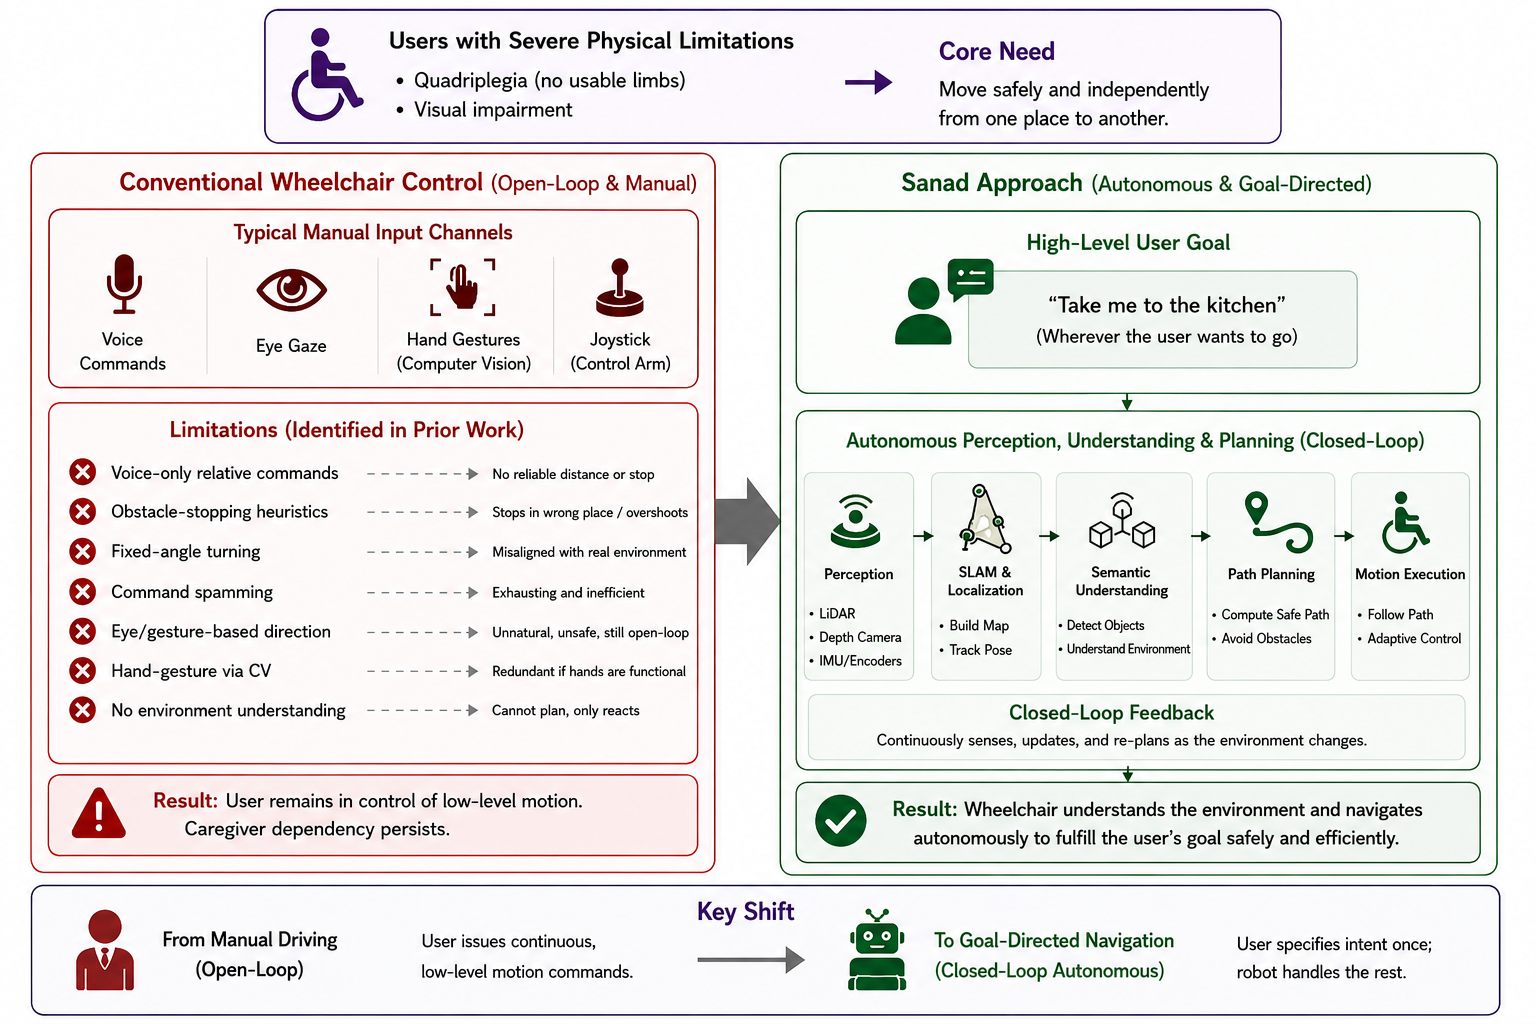
\includegraphics[width=0.75\textwidth]{figures/ch03/problem_statement_comparison.png}
    \caption{Manual/open-loop control (traditional and prior graduation projects) vs. Sanad's autonomous, goal-directed control model.}
    \label{fig:problem_statement_comparison}
\end{figure}

\section{Statistics \& Numbers}

The scale of the problem Sanad addresses is significant both globally and locally:

\begin{itemize}
    \item The World Health Organization estimates that approximately \textbf{80 million people worldwide} (roughly 1\% of the global population) require a wheelchair for mobility, and that this number continues to grow due to population aging, spinal cord injuries, and chronic health conditions~\cite{who2023wheelchair}.
    \item In low- and middle-income countries, the gap between need and access is especially severe: an estimated \textbf{60--75\% of people who need a wheelchair do not have access to one} appropriate for their condition, due to cost, import duties, and limited distribution infrastructure~\cite{ameco2025wheelchairmarket, ncbi2024wheelchairprovision}.
    \item In \textbf{Egypt}, estimates of the number of people living with disabilities vary widely depending on the source and methodology, ranging from around \textbf{2.4 million} (2006 national census, 1.8\% of the population) to \textbf{12--15 million} (UNDP / National Academy for Information Technology for Persons with Disabilities estimates, roughly 8.8--15\% of the population)~\cite{wikipedia2023disabilityegypt, egyptianstreets2024disability, naid2026about}. A 2018 AUC report indicates that around \textbf{15\% of Egyptians with disabilities} have a physical impairment, a subset of which corresponds to wheelchair-dependent individuals.
    \item Among wheelchair users specifically, a meaningful fraction have \textbf{quadriplegia or equivalent total-mobility loss} (e.g., due to spinal cord injury, ALS, cerebral palsy, or stroke), and a smaller but non-trivial fraction are additionally visually impaired --- both groups fall entirely outside what a manual joystick-controlled chair can serve.
    \item Recent published research on ROS-based voice-controlled smart wheelchairs reports mean localization errors below 10~cm and goal-completion rates around 94\% using LiDAR SLAM and AMCL localization~\cite{benayed2026voicecontrolled} --- figures that confirm the technical feasibility of the autonomous, SLAM-based approach Sanad adopts, and serve as a useful benchmark for Sanad's own evaluation.
\end{itemize}


\section{Gap in the Market}

Sanad's positioning becomes clear once the landscape is compared layer by layer: commercial products, international research, and local (Egyptian) graduation projects. Table~\ref{table:gap_summary} summarizes what each layer already offers and what it is still missing.
\begin{table}[H]
\centering
\caption{Summary of the market/research gap across commercial, international, and local layers.}
\label{tab:market_gap}

\begin{tabular}{|>{\raggedright\arraybackslash}p{2.8cm}|
                >{\raggedright\arraybackslash}p{5.4cm}|
                >{\raggedright\arraybackslash}p{5.4cm}|}
\hline
\textbf{Layer} & \textbf{What exists} & \textbf{What's missing} \\
\hline

\textbf{Commercial products}
\begin{itemize}[leftmargin=*,nosep]
    \item WHILL
    \item LUCI
    \item DROVE
\end{itemize}
&
\begin{itemize}[leftmargin=*,nosep]
    \item Proven autonomous driving and safety systems.
    \item Successfully deployed at scale (e.g., airports, retrofit kits).
\end{itemize}
&
\begin{itemize}[leftmargin=*,nosep]
    \item No support for users with zero limb or vision capability.
    \item Autonomy is limited to fixed, pre-mapped destinations.
\end{itemize}
\\
\hline

\textbf{International research}
\begin{itemize}[leftmargin=*,nosep]
    \item VAHM
    \item WAD
    \item CoNav Chair
    \item Benayed \& Masmoudi (2026)
\end{itemize}
&
\begin{itemize}[leftmargin=*,nosep]
    \item SLAM-based navigation.
    \item Voice control.
    \item Multimodal input techniques demonstrated individually.
\end{itemize}
&
\begin{itemize}[leftmargin=*,nosep]
    \item No single system integrates:
    \begin{itemize}[leftmargin=*,nosep]
        \item Full autonomous navigation.
        \item Eye tracking.
        \item Smart-home control.
        \item Remote communication.
    \end{itemize}
\end{itemize}
\\
\hline

\textbf{Egyptian graduation projects}
\begin{itemize}[leftmargin=*,nosep]
    \item ITIDA projects~\cite{itida2021gradprojects}
\end{itemize}
&
\begin{itemize}[leftmargin=*,nosep]
    \item Voice-controlled wheelchair prototypes.
    \item EEG-controlled wheelchair prototypes.
    \item Eye-movement-controlled wheelchair prototypes.
\end{itemize}
&
\begin{itemize}[leftmargin=*,nosep]
    \item All remain manual/open-loop.
    \item None perform autonomous mapping or path planning.
\end{itemize}
\\
\hline

\end{tabular}
\end{table}

The pattern repeats at every layer: autonomous navigation and fully accessible, no-limb/no-vision control have each been demonstrated separately, but never combined --- together with smart-home integration and independent caregiver communication --- into a single home-use platform. This is precisely the combination Sanad is designed to deliver, and it is the basis for the ``What is Sanad?'' description in the next section.

\section{What is Sanad?}

Sanad is an \textbf{autonomous, ROS~2-based smart wheelchair} designed for users with severe mobility impairments, including quadriplegia and visual impairment. Unlike traditional powered wheelchairs, Sanad builds a live map of its environment using LiDAR-based SLAM and localizes itself within that map using AMCL, allowing it to plan and execute paths to a destination on its own once the user specifies a high-level goal, instead of requiring continuous manual steering.

The system is organized around several integrated capabilities:

\begin{itemize}
    \item \textbf{Autonomous indoor navigation}: SLAM Toolbox for mapping, AMCL for localization, and Nav2 for path planning and obstacle avoidance, so that a command such as ``go to the kitchen'' is executed end-to-end without further input from the user.
    \item \textbf{Multi-modal, accessibility-first input}: the primary interaction channel is natural-language voice control (in Arabic), interpreted through an LLM-based intent router. For users who retain some hand mobility, a touch-screen interface is available as a faster alternative. For users who cannot speak or use their hands at all, an \textbf{eye-tracking} interface allows navigation and control purely through gaze. A camera-based \textbf{head-tilt/IMU} controller additionally allows fine, low-speed maneuvering once the chair has reached a room.
    \item \textbf{Vision-Language Model (VLM) assisted navigation}: rather than requiring a pre-labeled destination, a user can describe an object or place in natural language (e.g., ``take me next to the fridge''), and a depth camera combined with a VLM locates the target within the observed scene and provides a navigation goal to the planner.
    \item \textbf{Smart-home control}: integration with home appliances (lighting, television, air conditioning, etc.) via IR blasters and network-connected devices, so the same voice/eye/touch interface that controls mobility also controls the user's immediate environment.
    \item \textbf{Remote communication}: a Telegram-based module allows the user to dictate and autonomously send messages to family members or caregivers without assistance, restoring a channel of independent communication.
    \item \textbf{Natural-language text-to-speech feedback}: Gemini-based TTS provides spoken confirmations and responses, closing the interaction loop for users who cannot read a screen.
\end{itemize}

\begin{figure}[H]
    \centering
    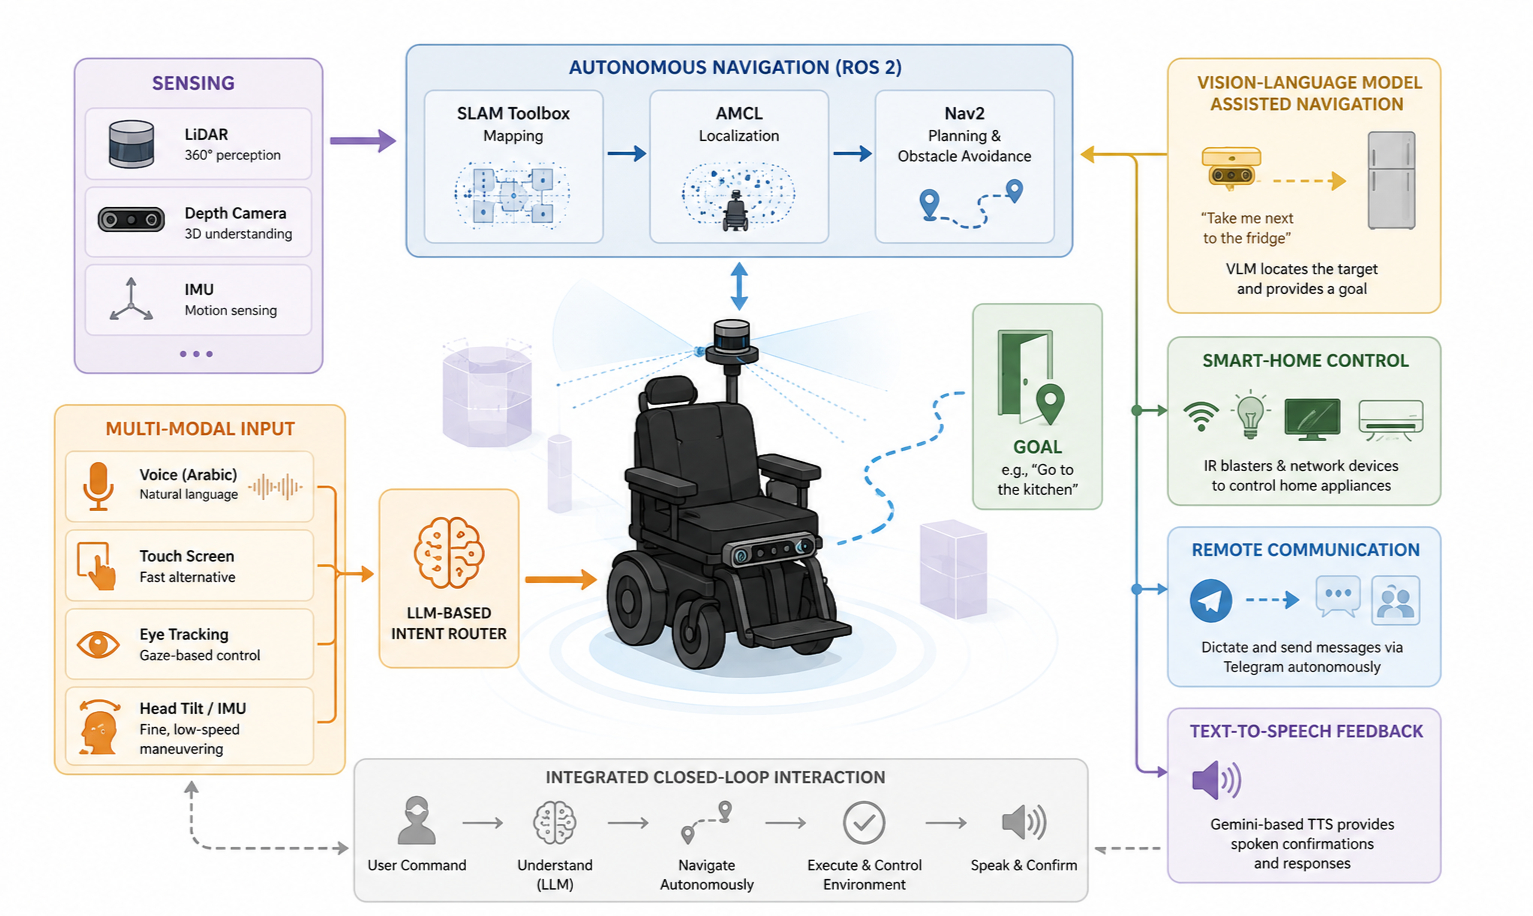
\includegraphics[width=0.8\textwidth]{figures/ch03/sanad_system_overview.png}
    \caption{High-level overview of the Sanad system: sensing, autonomous navigation, and multi-modal control/communication modules.}
    \label{fig:sanad_overview}
\end{figure}

\section{Target Users}

Sanad is designed primarily for:

\begin{itemize}
    \item \textbf{Individuals with quadriplegia} or equivalent total/near-total loss of limb mobility (e.g., due to spinal cord injury, advanced ALS, severe cerebral palsy, or stroke), who cannot operate a joystick or manual control arm.
    \item \textbf{Users with combined mobility and visual impairment}, who cannot rely on sight to judge distances, doorways, or obstacles even if an alternative manual input were available to them.
    \item \textbf{Users with limited or no speech}, who can still interact with Sanad through the eye-tracking interface.
    \item Secondarily, \textbf{users with partial hand mobility} who benefit from the touch-screen interface as a faster alternative to full manual driving, and their \textbf{caregivers}, who benefit from reduced supervision requirements and from the smart-home and communication features.
\end{itemize}


\begin{table}[H]
\centering
\caption{Representative user profiles considered during the requirements analysis.}
\label{tab:user_personas}
\renewcommand{\arraystretch}{1.4}

\begin{tabularx}{\textwidth}{|>{\centering\arraybackslash}p{1.8cm}|
                                >{\raggedright\arraybackslash}p{2.8cm}|
                                >{\raggedright\arraybackslash}X|
                                >{\raggedright\arraybackslash}X|
                                >{\raggedright\arraybackslash}X|}
\hline
\textbf{User Profile} &
\textbf{Disability} &
\textbf{Control Method} &
\textbf{Primary Need} &
\textbf{Relevant Sanad Features} \\
\hline

Profile 1 &
Quadriplegia &
Voice commands or IMU-based head control &
Independent mobility without hand movement &
Autonomous navigation, obstacle avoidance, voice interface, and head-motion control. \\
\hline

Profile 2 &
Quadriplegia with visual impairment &
Voice commands &
Safe navigation without visual feedback &
Autonomous navigation, voice interface, obstacle avoidance, and audio feedback. \\
\hline

Profile 3 &
Complete paralysis with speech impairment &
Eye tracking &
Hands-free and speech-free wheelchair control &
Eye-tracking interface, autonomous navigation, and obstacle avoidance. \\
\hline

Profile 4 &
Lower-limb disability &
Touchscreen interface &
Comfortable navigation with minimal manual driving &
Touchscreen destination selection, autonomous navigation, and smart home integration. \\
\hline

\end{tabularx}
\end{table}

\noindent\textbf{Note:} Profile~4 is capable of operating a conventional powered wheelchair using manual controls. However, this user chooses \textit{Sanad} to benefit from autonomous navigation, easier movement within the home environment, and reduced physical effort compared to continuous manual control.

\section{Summary and Transition}
This chapter has outlined the design space and objectives of the Sanad assistive wheelchair, framing it as an autonomous solution to manual-control limitations. The next chapter, Chapter 2 (Literature Review and Market Analysis), builds upon this context by analyzing existing academic research and benchmarking commercial offerings to locate Sanad within the state of the art.